% IEEE conference format (IEEEtran). Build: see docs/paper/ieee/README.md
\documentclass[conference]{IEEEtran}
\IEEEoverridecommandlockouts
\usepackage{cite}
\usepackage{amsmath,amssymb}
\usepackage{graphicx}
\usepackage{booktabs}
\usepackage{array}
\usepackage{textcomp}
\usepackage{url}
\usepackage{balance}
\def\BibTeX{{\rm B\kern-.05em{\sc i\kern-.025em b}\kern-.08em T\kern-.1667em\lower.7ex\hbox{E}\kern-.125emX}}
\newcommand{\pass}{\textsc{pass}}
\newcommand{\fail}{\textsc{fail}}
\newcommand{\na}{\textsc{na}}
\newcommand{\ctl}[1]{\texttt{#1}}

\begin{document}

\title{A Taxonomy-Driven Security Assessment Framework for KVM Virtualization: Configuration Auditing, Attack-Path Modelling and Real-Host Evaluation}

\author{\IEEEauthorblockN{A. Doni Aditya (23BDS007), B. Harsha Vardan (23BDS015), E. Hariteja (23BDS019), and L. Sahith Akash Manikanta (23BDS031)}
\IEEEauthorblockA{Course project, Cloud Security \& Vulnerabilities, submitted to Malay Kumar}}

\maketitle

\begin{abstract}
Security knowledge about virtualization is spread over survey prose and generic hardening checklists, and neither says which attack a misconfiguration enables, how far a breach spreads, or what to fix first. We present \emph{vsec}, a taxonomy-driven assessment framework for KVM/libvirt/QEMU hosts. It turns the threat taxonomy of a 2020 virtualization-security survey into 31 controls in nine threat classes, each traced to a survey section, and implements a configuration auditor, a snapshot secret scanner, a memory-forensics checker and a hypervisor-detection design. A new attack-path layer models 11 survey attacks as staged chains whose stages are stopped by named audit results; it shows how a breach spreads across VMs and hosts and computes the smallest set of fixes that blocks every modelled attack. We evaluate on constructed inputs with known ground truth and on one real KVM host. The auditor matched all 10,400 seeded decisions in 400 folders. A weakness we found in our own scanner (0/120 encoded secrets found) was closed by decoding passes (80/120 on fresh data; secrets split across pages remain undetected). On the real host, a stock installation failed 8 of 28 configuration controls and 2 after the printed fixes, both platform limits, while Lynis checked none of these settings; a real memory snapshot leaked all 11 planted secrets and the improved scanner found all of them. In the model, a VM on a fully hardened host was breached in up to 46.9\% of random fleets unless its own settings were hardened too. The attack-path layer is a model of the survey's logic, not a measurement of real attacks.
\end{abstract}

\begin{IEEEkeywords}
KVM, virtualization security, security taxonomy, configuration auditing, attack-path modelling, memory forensics
\end{IEEEkeywords}

\section{Introduction}
KVM with QEMU and libvirt is widely used to run cloud virtual machines (VMs). Its attack surface is wide: emulated devices run with hypervisor privilege, the management plane is reachable over sockets and the network, VMs share hardware caches and memory pages, and memory snapshots contain everything the guest knew. A 2020 survey by Sierra-Arriaga et al.\ \cite{survey} organises this surface into a taxonomy of threat classes, but a survey is text: it cannot be run against a system. Hardening tools such as Lynis \cite{lynis}, OpenSCAP \cite{openscap} and the CIS benchmarks \cite{cis} can be run, but they report a flat list of settings. An administrator facing a long list of failing settings cannot tell which attack each one enables, which VMs are put at risk, or which fix to apply first.

We ask three research questions.
\textbf{RQ1:} Can the survey's taxonomy be turned into checkable controls that remain traceable to the survey?
\textbf{RQ2:} Can audit results be connected to the survey's attack chains so that the spread of a breach and the priority of fixes become visible?
\textbf{RQ3:} How reliable are the checks, and what do they find on a real KVM host?

\noindent The contributions of this paper are:
\begin{enumerate}
\item A taxonomy of 31 controls in nine threat classes, each traced to a survey section, with explicit semantics for results that cannot be determined (\na{} is never counted as \pass).
\item \emph{vsec}, an implementation with four modules: a configuration auditor (28 controls), a snapshot secret scanner with redaction, a memory-forensics check and a hypervisor-detection design.
\item An attack-path model that links audit results to 11 survey attacks, simulates the spread of a breach across a fleet of hosts and VMs, and computes the exact smallest fix set.
\item An evaluation consisting of six reproducible experiments and a real-host study (audit before and after hardening, comparison with Lynis, real memory snapshot), including a weakness found and fixed in our own scanner.
\end{enumerate}
The work contains no exploit code. Section~\ref{sec:valid} states what the results do and do not show.

\section{Background and Related Work}
\subsection{Virtualization Threats}
The survey \cite{survey} groups attacks by the boundary they cross: guest to host, host to hypervisor, guest to guest, side channels, DMA through devices, snapshot privacy, introspection and hypervisor-presence attacks. Representative cases include the QEMU floppy-controller flaw (VENOM, CVE-2015-3456) \cite{venom}, memory-deduplication timing channels \cite{suzaki}, Rowhammer combined with deduplication \cite{razavi}, transient-execution leaks \cite{kocher,vanbulck} and DMA attacks through peripherals \cite{markettos}. Hypervisor memory forensics \cite{graziano} and VMM detection \cite{garfinkel,raffetseder} cover the last two classes.

\subsection{Hardening and Compliance Tools}
Lynis \cite{lynis}, OpenSCAP \cite{openscap} and the CIS benchmarks \cite{cis} audit operating-system and service configuration against checklists. They do not relate findings to the survey's attack taxonomy, and (as Section~\ref{sec:real} shows) Lynis has no check for QEMU or VM settings.

\subsection{Attack Graphs and Trees}
Attack trees \cite{schneier} and attack graphs \cite{sheyner,mulval} model how an attacker combines weaknesses. We use the same idea in a restricted, data-driven form: each attack is a short chain whose stages are gated by taxonomy controls, and the chains are evaluated on real audit results of a fleet.

\begin{table}[!t]
\caption{Capabilities of existing practice and vsec}
\label{tab:compare}
\centering\footnotesize
\begin{tabular}{@{}p{3.55cm}ccc@{}}
\toprule
Capability & Checklists & Survey & vsec \\
\midrule
Checks real host/VM configuration & Yes & No & Yes \\
Check traced to a survey class & No & n/a & Yes \\
Attacks as stages gated by controls & No & Prose & Yes \\
Spread across VMs and hosts & No & Prose & Yes \\
Fixes ranked, exact smallest set & No & No & Yes \\
Defence in depth per attack & No & No & Yes \\
Reports \na{} instead of guessing & Partly & n/a & Always \\
\bottomrule
\end{tabular}
\end{table}

Table~\ref{tab:compare} compares capabilities as documented by the tools' stated purpose; it is not a benchmark. The new element is the attack-chain layer on top of real audit results.

\section{The vsec Framework}
\subsection{Taxonomy and Controls}
Table~\ref{tab:tax} lists the nine threat classes. Every control has an identifier, a test, the expected value, a fix command and a reference to the survey section; the mapping is part of the repository (\texttt{taxonomy.yaml}). Controls carry one of three labels: \emph{Tested} (a live probe), \emph{Config-proxy} (configuration or version check only) and \emph{Tested on E1} (needs bare-metal hardware).

\begin{table}[!t]
\caption{Threat classes and controls (31 in total)}
\label{tab:tax}
\centering\footnotesize
\begin{tabular}{@{}p{2.15cm}cp{3.1cm}p{1.15cm}@{}}
\toprule
Class & \# & Example controls & Label \\
\midrule
Guest$\to$Host & 12 & seccomp, sVirt, non-root QEMU, console, devices & Tested \\
Host$\to$VMM & 6 & image/socket permissions, libvirt TCP & Config \\
Side channels & 3 & KSM off, CPU mitigations, SMT & Config \\
Guest$\to$Guest & 3 & network mode, reachability, shared memory & Config \\
DMA/IOMMU & 2 & IOMMU on, IOMMU groups & On E1 \\
VMM vulnerabilities & 2 & QEMU / kernel CVE lists & Config \\
Snapshot privacy & 1 & secrets in memory dump (M2) & Tested \\
Hidden processes & 1 & process views differ (M3) & Tested \\
Hypervisor presence & 1 & multi-signal detection (M4) & Tested \\
\bottomrule
\end{tabular}
\end{table}

\subsection{Result Semantics}
Each control returns \pass, \fail{} or \na{} with the evidence string. \na{} means the check could not run or could not be trusted (for example the IOMMU test inside WSL2, or a CVE list that is not verified); it is never converted to \pass. A check that raises an error is reported as \na. A \pass{} means that the control passed its defined test, not that the system is secure.

\subsection{Modules}
\textbf{M1, configuration auditor.} It reads files captured by \texttt{vsec collect} (libvirt domain XML, \texttt{qemu.conf}, \texttt{libvirtd.conf}, kernel command line, sysfs vulnerability status, file permissions, versions) and evaluates 28 controls. The collector redacts passwords and secrets before writing and drops any file it cannot verify as clean. \textbf{M2, snapshot scanner.} It scans a memory dump with rules for private keys, AWS key pairs, JWTs and 64-hex tokens, filters low-entropy hex, and redacts matches in place by zeroing (same size). \textbf{M3} compares process views of a memory image with Volatility~3 \cite{volatility} to find hidden processes. \textbf{M4} is a pre-specified design for detecting a hidden hypervisor from timing and scheduling signals; it is not evaluated in this paper. Fig.~\ref{fig:arch} shows the architecture.

\begin{figure*}[!t]
\centering
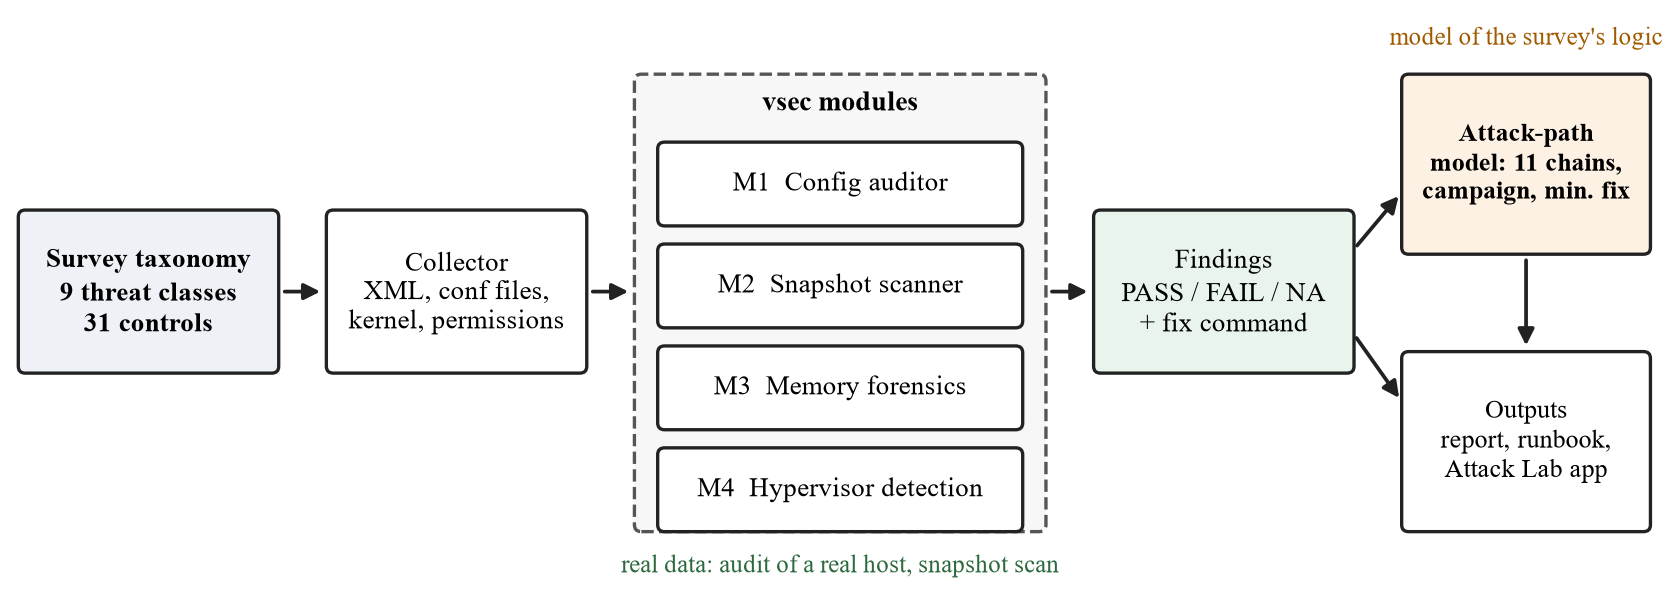
\includegraphics[width=0.92\textwidth]{figs/fig_arch.png}
\caption{Architecture of vsec. Real data flows from the collector through the modules into findings; the attack-path model applies the survey's logic to those findings.}
\label{fig:arch}
\end{figure*}

\section{Attack-Path Model}
\subsection{Single VM}
Let $C$ be the set of controls and $\sigma: C\to\{\pass,\fail,\na\}$ the audit state of a VM. An attack $a$ is a sequence of stages $s_1,\dots,s_n$; stage $s_i$ has a gate set $G_i\subseteq C$ taken from the survey's description (possibly empty, meaning the underlying flaw is assumed). Stage $i$ is stopped when
\begin{equation}
\exists g\in G_i:\ \sigma(g)=\pass .
\end{equation}
The attack is \emph{blocked} at the first stopped stage and \emph{open} if no stage is stopped. The defence depth is the number of distinct passing gates on its path,
\begin{equation}
d(a,\sigma)=\Bigl|\{\,g\in\textstyle\bigcup_i G_i:\sigma(g)=\pass\,\}\Bigr| ,
\end{equation}
and the risk score of a VM, with $O(\sigma)$ the open attacks and $\mathrm{sev}(a)\in\{1..4\}$ the severity, is
\begin{equation}
R(\sigma)=100\cdot\frac{\sum_{a\in O(\sigma)}\mathrm{sev}(a)}{\sum_{a\in A}\mathrm{sev}(a)} .
\end{equation}
Table~\ref{tab:attacks} lists the 11 attacks. Severity, origin and reach are our own judgement; the stage structure follows the survey text.

\begin{table*}[!t]
\caption{Attacks in the model (origin: who can start it; reach: what a success gives; gates: controls that stop a stage, a semicolon separates stages)}
\label{tab:attacks}
\centering\footnotesize
\begin{tabular}{@{}llllllll@{}}
\toprule
ID & Attack & Class & Sev. & Origin & Reach & Survey & Gate controls \\
\midrule
A01 & Floppy-controller escape (VENOM-style) & Guest$\to$Host & 4 & guest & host & S4.1 & C14; C03, C04; C05, C06; C07, C08 \\
A02 & Open VNC/SPICE console takeover & Guest$\to$Host & 3 & network & VM & S2.1, S5.2 & C12; C11 \\
A03 & Unauthenticated libvirt over TCP & Host$\to$VMM & 4 & network & host & S3.1, S5.2 & C20 \\
A04 & World-writable libvirt socket & Host$\to$VMM & 4 & local & host & S3.1, S5.2 & C18, C19 \\
A05 & Memory-deduplication timing channel & Side channels & 2 & guest & leak & S5.4.3 & C09 \\
A06 & Rowhammer + deduplication & Side channels & 3 & guest & leak & S4.2 & C09 \\
A07 & Transient-execution read & Side channels & 3 & guest & leak & S5.4.5 & C25; C26 \\
A08 & Malicious DMA from a device & DMA/IOMMU & 4 & guest & host & S5.1, S5.3 & C01, C02 \\
A09 & Secret theft from VM snapshots & Snapshot & 3 & local & VM & S6.1.1 & C21; C17 \\
A10 & Neighbour VM pivot over shared network & Guest$\to$Guest & 3 & guest & neighbour & S3.1, S4.2 & C15; C16 \\
A11 & Rogue hypervisor inside a guest & Hypervisor & 3 & guest & VM & S7.1, S7.2 & C10 \\
\bottomrule
\end{tabular}
\end{table*}

\subsection{Fleet and Campaign}
A fleet has hosts $H$ and VMs $V$; each VM has a host $h(v)$, a network segment and a criticality $\mathrm{crit}(v)\in\{1,2,3\}$. Eight controls live in a VM's own libvirt definition (console, devices, network, shared memory, cache) and belong to the VM; all other controls belong to the host and are \emph{shared by every VM on it}, so the state seen by $v$ is $\sigma_v=\sigma_{h(v)}\cup\sigma^{\mathrm{vm}}_v$. A \emph{campaign} starts with an outsider or with root in one VM and applies explicit rules. A network-origin attack is tried against every VM once. From a compromised VM $x$, a guest-origin attack with reach \emph{host} compromises every VM on $h(x)$; with reach \emph{neighbour} it compromises a VM $y$ on the same segment if it is open on both $x$ and $y$; with reach \emph{leak} it exposes the data of co-resident VMs; reach \emph{VM} records persistence only. The blast radius, with $K$ the set of compromised VMs, is
\begin{equation}
B=100\cdot\frac{\sum_{v\in K}\mathrm{crit}(v)}{\sum_{v\in V}\mathrm{crit}(v)} .
\end{equation}

\subsection{Fix Planning}
For a VM the \emph{minimal fix set} is the smallest $F\subseteq\{g:\sigma(g)=\fail\}$ with $F\cap G(a)\neq\emptyset$ for every open attack $a$, where $G(a)=\bigcup_i G_i$; this is a minimum hitting set, solved exactly by branch and bound (branching on the open attack with the fewest candidate gates). Gates in state \na{} are not counted as fixable. For a campaign the tool ranks single fixes by how much they reduce the number of compromised VMs, and falls back to pairs when two independent paths are open.

\begin{figure*}[!t]
\centering
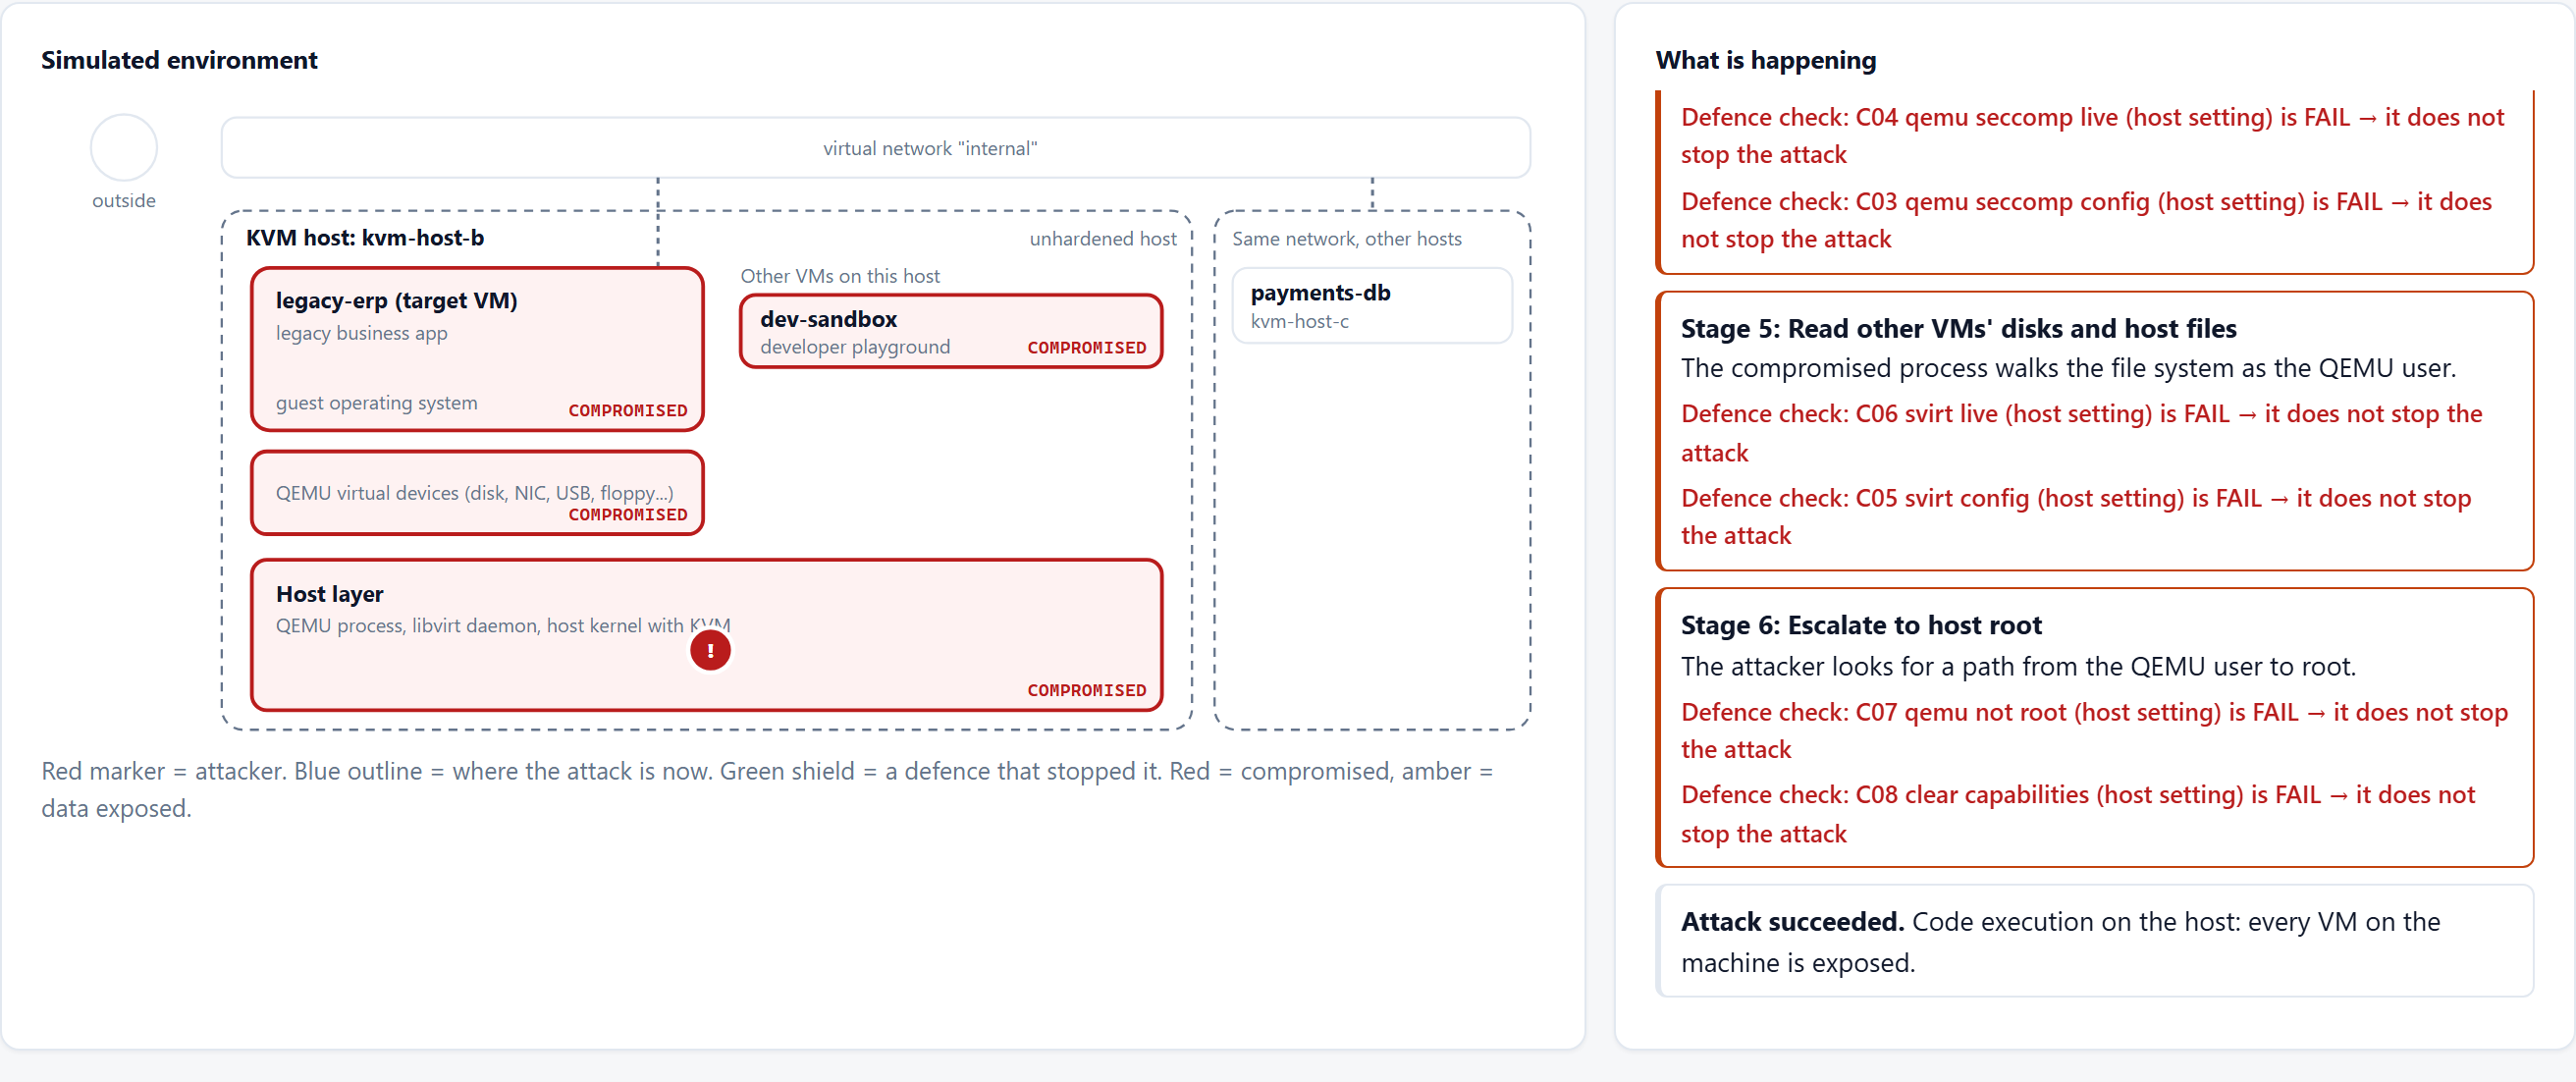
\includegraphics[width=0.95\textwidth]{figs/fig_sim.png}
\caption{Attack Lab: the floppy-controller escape against a VM on an unhardened host. Each stage and its defence check are shown; the host layer and the other VM on the host end as compromised. Applying one fix (C14) blocks the attack at stage~2.}
\label{fig:sim}
\end{figure*}

\section{Implementation}
vsec is a Python 3.12 package with a command-line interface (\texttt{run}, \texttt{audit}, \texttt{pilot}, \texttt{m3}) and a collector (\texttt{vsec.collect}) that captures host files on the KVM host. The taxonomy, the attack chains and the example fleet are data files (\texttt{taxonomy.yaml}, \texttt{attacks.yaml}, \texttt{fleet.yaml}), so changing a rule does not require code changes. The Attack Lab is a self-contained single-file web application (\texttt{simulator.html}) with a guided four-step view (choose a VM, choose an attack, watch the staged simulation, see how to protect) and tabs for fleet overview, per-VM insights, campaigns, a hardening challenge and a survey map. Its JavaScript engine mirrors the Python engine; a test compares posture, risk, minimal fix, campaign and containment advice on 25 random fleet states. The page can import a real audit. The suite has 1,037 passing tests (20 are Linux-only and skipped on Windows). All experiments run from fixed seeds with one command (\texttt{run\_experiments.py}, about 70\,s). No exploit code exists in the repository, planted secrets are random fake values, and memory dumps are deleted after use.

\section{Experimental Design}
\subsection{Constructed-Input Experiments}
\textbf{E1} breaks each of the 26 testable controls in each of three seeded variants, one at a time, in an otherwise hardened case folder (78 cases; the two CVE controls are \na{} by design). \textbf{E2} generates 400 folders in which each control is broken independently with probability $p\in\{0.1,0.3,0.5,0.7\}$ (100 folders each); every control in every folder is one decision. \textbf{E3} generates 260 synthetic memory dumps (256\,KiB) with secrets of four types planted in live, freed and exited memory, plus three held-out encodings (UTF-16LE, base64, split across pages) and negative dumps. The scanner version evaluated after a fix (v2) is scored on newly generated dumps.

\subsection{Model Experiments}
On the example fleet (6 VMs on 3 hosts, one host fully hardened) we compute \textbf{E4}, the control leverage (open VM--attack pairs blocked when one control is fixed everywhere) and the greedy containment of an outsider; \textbf{E5}, a Monte Carlo study of 2,000 random fleets per cell in which every control outside the hardened host fails with probability $p$; and \textbf{E6}, the share of blocked attacks that rely on exactly one control.

\subsection{Real-Host Study}
The real host (environment E0) is a Windows~11 laptop (Intel Core i5-1155G7) running WSL2 (kernel 6.6.114.1) with Ubuntu 24.04.5, QEMU 8.2.2 and libvirt 10.0.0; \texttt{/dev/kvm} is available through nested virtualization and the guest is a hardware-accelerated KVM domain (CirrOS 0.6.2, 256\,MiB). One WSL2-specific setting was needed so that libvirt can start guests (\texttt{cgroup\_controllers = [ ]}). The guest was audited three times: as created by a stock \texttt{virt-install}; after we added three misconfigurations that survey attacks rely on (a floppy controller, VNC on all interfaces, unsafe disk cache); and after applying the fix commands the audit printed. Lynis 3.0.9 was run on the same host. For the snapshot test we planted fake secrets in the running guest over its serial console, as plain text, base64 and UTF-16LE, took a real snapshot with \texttt{virsh dump --memory-only}, and scanned and redacted it. Metrics are precision, recall, false-positive rate and 95\% Wilson intervals \cite{wilson}.

\section{Results and Analysis}
\subsection{Auditor Accuracy (E1, E2)}
All 78 single-fault cases were detected (95\% CI 95.3--100\%) and in none did another control change state. In E2 the auditor made 10,400 decisions (4,058 true positives, 6,342 true negatives, no false positives or negatives), so precision and recall are 100\% with a 95\% lower bound of 99.9\%; every one of the 400 folders was exactly right, at every fault rate. One audit took 40.3\,ms (median; 72.8\,ms at the 95th percentile). Because the same team wrote the checks and the faults, this shows that the checks behave as specified and do not interfere with each other even when up to 70\% of controls are broken at once; it is not accuracy on real hosts.

\subsection{Snapshot Scanner (E3)}
\begin{table}[!t]
\caption{Scanner on synthetic dumps (secrets found / present)}
\label{tab:m2}
\centering\footnotesize
\begin{tabular}{@{}lccc@{}}
\toprule
Storage form & v1 & v2 (decoding) & Real dump v1 / v2 \\
\midrule
Plain text & 120/120 & 120/120 & 4/4 \; 4/4 \\
UTF-16LE & 0/40 & 40/40 & 0/3 \; 3/3 \\
Base64 & 0/40 & 40/40 & 0/4 \; 4/4 \\
Split across pages & 0/40 & 0/40 & -- \\
\midrule
False positives & 0 & 0 & 13 \; 13 \\
\bottomrule
\end{tabular}
\end{table}
Scanner v1 found every plainly stored secret with no false positives and none of the encoded ones (Table~\ref{tab:m2}), a weakness that the held-out design was built to expose. We added decoding passes for UTF-16LE text and base64 runs (v2) and scored v2 on freshly generated dumps: all UTF-16LE and base64 secrets are found, still with no false positives (80/120 held-out, 66.7\%, CI 57.8--74.5\%). Secrets split across pages remain undetected because no single place in memory holds the whole secret. After v2 redaction, all 240 planted dumps rescanned clean and the size was unchanged.

\subsection{Attack-Path Model (E4--E6)}
In the example fleet 27 of 66 (VM, attack) pairs are open. Fig.~\ref{fig:lev} shows the leverage of single fixes: turning off KSM (C09) blocks 8 open pairs, because it gates both the deduplication channel and Rowhammer with deduplication, and the two VM network settings C15 and C16 block 5 each. Two well-chosen fixes stop the outsider campaign completely (5, then 2, then 0 compromised VMs). The minimal fix set blocking all 11 attacks has 6, 5, 6, 5, 1 and 0 controls for the six VMs.

\begin{figure}[!t]
\centering
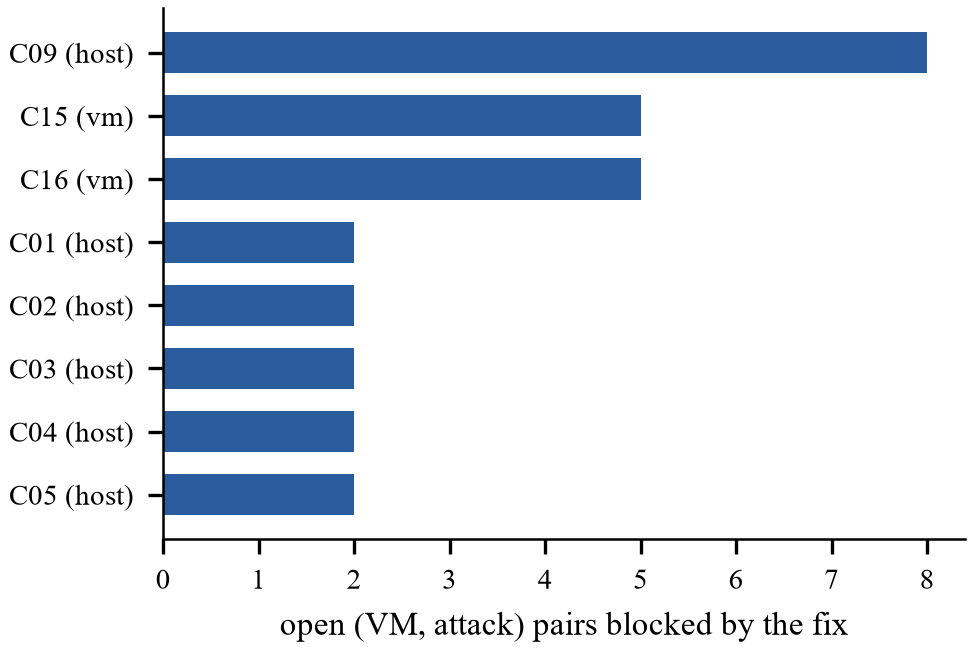
\includegraphics[width=\columnwidth]{figs/fig_leverage.png}
\caption{Control leverage in the example fleet (model): open (VM, attack) pairs blocked by fixing one control everywhere it fails.}
\label{fig:lev}
\end{figure}

Fig.~\ref{fig:hard} answers whether a hardened host is enough. With the host fully hardened but its VMs left to chance, an outsider still compromises at least one VM on that host in 1.8\%, 7.4\%, 17.8\% and 46.9\% of fleets at fault rates 0.1, 0.2, 0.3 and 0.5 (Wilson bands in the figure), through a VM's own network and console settings. When the host's VMs are hardened as well, the rate is 0\% in all 8,000 fleets (upper bound 0.2\% per cell), and isolating every network adds nothing further for those VMs. Finally, 15,983 of 27,901 blocked pairs (57.3\%, CI 56.7--57.9\%) are held by a single control, so one more misconfiguration would open them.

\begin{figure}[!t]
\centering
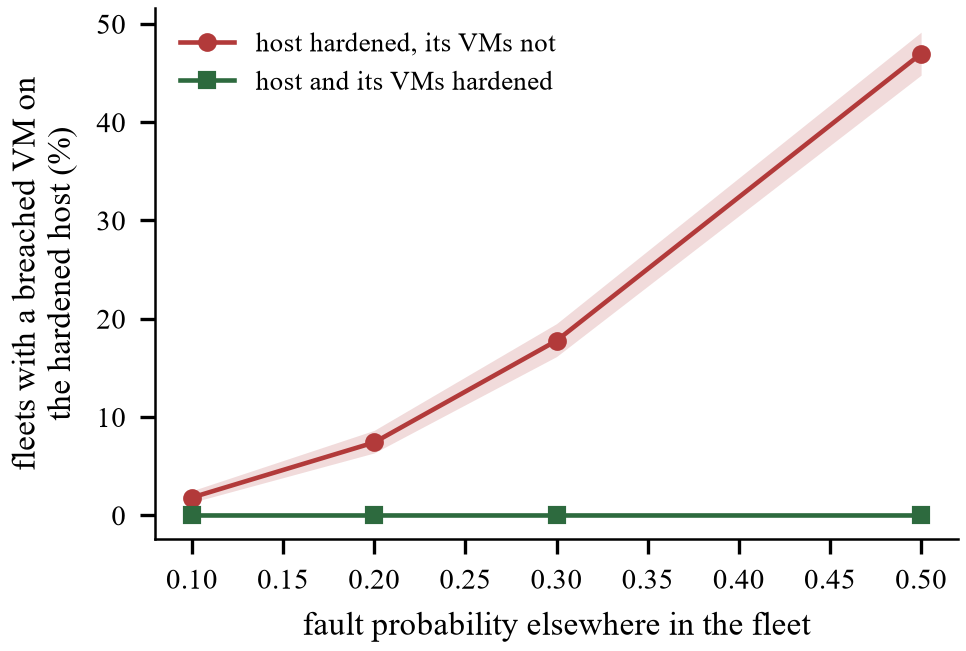
\includegraphics[width=\columnwidth]{figs/fig_hardhost.png}
\caption{Fleets in which a VM on the fully hardened host is breached, with 95\% Wilson bands (model, 2,000 fleets per point).}
\label{fig:hard}
\end{figure}

\subsection{Real KVM Host}\label{sec:real}
\begin{table}[!t]
\caption{Real host: the same guest audited three times (28 controls)}
\label{tab:real}
\centering\footnotesize
\begin{tabular}{@{}lcccp{2.5cm}@{}}
\toprule
Audit & \fail & \pass & \na & Failing controls \\
\midrule
Stock install & 8 & 15 & 5 & C01 C06 C10 C11 C15 C16 C17 C21 \\
After weakening & 11 & 12 & 5 & + C12 C14 C22 \\
After printed fixes & 2 & 22 & 4 & C01 C06 \\
\bottomrule
\end{tabular}
\end{table}
A stock installation already fails 8 controls (Table~\ref{tab:real}): the VNC console has no password (C11), the guest sits on the NAT network with a host-side channel (C15, C16), the disk image and the save and dump directories are world-readable (C17, C21) and nested virtualization is on (C10). All three seeded weaknesses were detected (C12, C14, C22 turned \fail), and every failing control that a configuration change can fix turned \pass{} after the printed fix. The two that remain are platform limits: WSL2 has no IOMMU on the kernel command line (C01) and no AppArmor or SELinux, so QEMU runs unconfined (C06); IOMMU groups are \na{} on E0. During hardening, C16 failed once more because our ``isolated'' network still had an IP address, which gives the guest a path to services on the host bridge; vsec reported it and the fix passed. Lynis ran 247 tests (hardening index 64). Its virtualization-related output is limited to systemd exposure ratings for \texttt{libvirtd}, \texttt{virtlockd} and \texttt{virtlogd} (the first two rated UNSAFE) and a generic check for the presence of AppArmor or SELinux; its log contains no mention of QEMU, KVM, seccomp, KSM, nested virtualization or VNC/SPICE. The comparison is about coverage, not accuracy: the two tools check different things.

The real snapshot (272\,MiB, taken in 0.4\,s) leaked all 11 planted secrets; v1 found only the 4 stored as plain text and v2 found all 11 (Table~\ref{tab:m2}). A twelfth secret (a UTF-16 SSH key) never reached guest memory, because the serial console could not type it, and is excluded. Both versions reported 13 further hits, all from the 64-hex rule. We inspected five of them: they are public constants in the guest kernel (NIST P-256 curve parameters and the digits of $\pi/4$), which is the known limit of that rule. Scanning ran at 44.9\,MiB/s (v1) and 19.3\,MiB/s (v2). After v2 redaction no planted secret remained and the size was unchanged. One more leak path appeared during setup: secrets typed at a shell prompt were saved in the shell history and loaded into memory again after a reboot, so they end up in every later snapshot of that VM.

\section{Discussion and Threats to Validity}\label{sec:valid}
\textbf{What the results show.} The survey's taxonomy can be turned into checks that are exact on their fault model, cheap to run and traceable (RQ1). Putting attack chains on top of audit results exposes things a flat list cannot: one control (KSM) is worth more than eight others, a hardened host does not protect a badly attached VM, and most defences are a single layer deep (RQ2). On one real host the auditor works, its fixes remove the findings, a stock install is not hardened, a general hardening tool does not cover these settings, and a real snapshot leaks secrets that the scanner finds and removes (RQ3).

\textbf{Internal validity.} The same team wrote the checks and the injected faults, so a shared misunderstanding would go unnoticed; independent confirmation on more real hosts is needed. \textbf{Construct validity.} A \pass{} is not proof of security. The attack chains encode our reading of the survey (a stage without a control always succeeds, one passing control stops its stage), and severity, origin, reach and criticality are our judgement; E4--E6 therefore give the consequences of these rules, not real attack success rates. \textbf{External validity.} The real results come from one host on WSL2 under Hyper-V, with a small test guest; the example fleet is invented; IOMMU and AppArmor controls could not be tested; M3 on real dumps and the M4 timing study (which needs bare-metal Linux) are not done. \textbf{Conclusion validity.} Proportions carry 95\% Wilson intervals, runs use fixed seeds and can be repeated, and the M4 analysis plan is fixed in advance.

\section{Conclusion and Future Work}
We turned a virtualization-security survey into 31 traceable controls, a working auditor and scanner, and an attack-path model that shows how misconfigurations chain into breaches across a fleet and which fixes matter most. Six reproducible experiments and a real KVM host show that the tool behaves as specified, that a stock installation is far from hardened, and that a general hardening tool does not cover the settings the survey's attacks rely on. A weakness in our own scanner was found by the evaluation and fixed. Future work is to repeat the real-host study on native Linux and several hosts, to run M3 on real memory images and the pre-specified M4 timing experiment, to reassemble secrets split across pages, to add survey controls not yet covered (PCIe ACS, Secure Boot, memory encryption, cache partitioning) and to validate the attack chains against reported incidents.

\section*{Acknowledgment}
The authors used an AI coding assistant (Claude, Anthropic) to produce most of the code, tests and first drafts of the text and figures. The authors chose the topic and scope, defined the experiments, ran all reported experiments and take responsibility for the content. Code review was automated only; no person independently reviewed or reproduced the work. The code, scripts and result files for every number in this paper are part of the submission.

\balance
\begin{thebibliography}{99}
\bibitem{survey} F. Sierra-Arriaga, R. R. Branco, and B. Lee, ``Security issues and challenges for virtualization technologies,'' \emph{ACM Comput. Surv.}, vol. 53, no. 2, Art. 45, pp. 1--37, 2020, doi: 10.1145/3382190.
\bibitem{lynis} CISOfy, ``Lynis security auditing tool.'' [Online]. Available: \url{https://cisofy.com/lynis/}
\bibitem{openscap} OpenSCAP Project, ``Open Security Content Automation Protocol.'' [Online]. Available: \url{https://www.open-scap.org/}
\bibitem{cis} Center for Internet Security, ``CIS Benchmarks.'' [Online]. Available: \url{https://www.cisecurity.org/benchmarks}
\bibitem{venom} National Institute of Standards and Technology, ``CVE-2015-3456,'' National Vulnerability Database. [Online]. Available: \url{https://nvd.nist.gov/vuln/detail/CVE-2015-3456}
\bibitem{suzaki} K. Suzaki, K. Iijima, T. Yagi, and C. Artho, ``Memory deduplication as a threat to the guest OS,'' in \emph{Proc. 4th European Workshop on System Security (EuroSec)}, ACM, 2011.
\bibitem{razavi} K. Razavi, B. Gras, E. Bosman, B. Preneel, C. Giuffrida, and H. Bos, ``Flip Feng Shui: Hammering a needle in the software stack,'' in \emph{Proc. 25th USENIX Security Symp.}, 2016, pp. 1--18.
\bibitem{kocher} P. Kocher \emph{et al.}, ``Spectre attacks: Exploiting speculative execution,'' in \emph{Proc. IEEE Symp. Security and Privacy (S\&P)}, 2019.
\bibitem{vanbulck} J. Van Bulck \emph{et al.}, ``Foreshadow: Extracting the keys to the Intel SGX kingdom with transient out-of-order execution,'' in \emph{Proc. 27th USENIX Security Symp.}, 2018, pp. 991--1008.
\bibitem{markettos} A. T. Markettos \emph{et al.}, ``Thunderclap: Exploring vulnerabilities in operating system IOMMU protection via DMA from untrustworthy peripherals,'' in \emph{Proc. Network and Distributed System Security Symp. (NDSS)}, 2019.
\bibitem{graziano} M. Graziano, A. Lanzi, and D. Balzarotti, ``Hypervisor memory forensics,'' in \emph{Proc. Research in Attacks, Intrusions, and Defenses (RAID)}, Springer, 2013.
\bibitem{garfinkel} T. Garfinkel, K. Adams, A. Warfield, and J. Franklin, ``Compatibility is not transparency: VMM detection myths and realities,'' in \emph{Proc. 11th USENIX Workshop on Hot Topics in Operating Systems (HotOS XI)}, 2007.
\bibitem{raffetseder} T. Raffetseder, C. Kruegel, and E. Kirda, ``Detecting system emulators,'' in \emph{Information Security}, LNCS vol. 4779, Springer, 2007, pp. 1--18.
\bibitem{schneier} B. Schneier, ``Attack trees,'' \emph{Dr. Dobb's Journal}, vol. 24, no. 12, Dec. 1999.
\bibitem{sheyner} O. Sheyner, J. Haines, S. Jha, R. Lippmann, and J. M. Wing, ``Automated generation and analysis of attack graphs,'' in \emph{Proc. IEEE Symp. Security and Privacy}, 2002, pp. 273--284.
\bibitem{mulval} X. Ou, S. Govindavajhala, and A. W. Appel, ``MulVAL: A logic-based network security analyzer,'' in \emph{Proc. 14th USENIX Security Symp.}, 2005, pp. 113--128.
\bibitem{volatility} Volatility Foundation, ``Volatility 3.'' [Online]. Available: \url{https://github.com/volatilityfoundation/volatility3}
\bibitem{wilson} E. B. Wilson, ``Probable inference, the law of succession, and statistical inference,'' \emph{J. Amer. Statist. Assoc.}, vol. 22, no. 158, pp. 209--212, 1927.
\end{thebibliography}

\end{document}
